\chapter{Planos de Negócio e Instrumentos de Fomento Regional}
\label{cap:10}
\markboth{CAPÍTULO 10 — PLANOS DE NEGÓCIO E FOMENTO}{CAPÍTULO 10 — PLANOS DE NEGÓCIO E FOMENTO}

\noindent\tagTerritorio\ \tagAV{Base AV3}

\begin{capObjetivos}
  Ao concluir este capítulo, você será capaz de:
  \begin{enumerate}[leftmargin=1.5em, itemsep=2pt]
    \item Diferenciar a função contemporânea do Plano de Negócio completo, do Sumário Executivo e do \textit{Pitch Deck} conforme o interlocutor e o estágio do empreendimento.
    \item Mapear a \textbf{Escada do Capital} para Empreendimentos de Base Tecnológica (EBT), distinguindo recursos não dilutivos de capital societário (\textit{equity}) e crédito subsidiado.
    \item Identificar os principais instrumentos brasileiros e regionais de fomento à inovação (CNPq, FAPESB, FINEP, Programa Centelha, BNB/FNE Inovação e BNDES).
    \item Calcular indicadores de tração e fôlego financeiro: \textbf{MRR, \textit{Gross Burn Rate}, \textit{Net Burn Rate}, \textit{Runway}} em meses e prazo até o ponto de equilíbrio operacional.
  \end{enumerate}
\end{capObjetivos}

\begin{capRevisao}
  Recupere três elementos estruturantes dos capítulos anteriores:
  \begin{itemize}[leftmargin=1.5em, itemsep=2pt]
    \item \textbf{Vale da Morte Tecnológico (Cap. 7):} o intervalo entre TRL 4 e TRL 6 exige capital paciente capaz de suportar fluxos de caixa acumulados negativos antes da escala comercial.
    \item \textbf{Dimensionamento TAM/SAM/SOM (Cap. 8):} agências de fomento e investidores avaliam a coerência entre o montante solicitado e o mercado alcançável (\textit{bottom-up}).
    \item \textbf{Economia Unitária (Cap. 9):} antes de buscar capital de risco ou crédito de expansão, a empresa precisa demonstrar validação do MVP e relação $\text{LTV/CAC} \ge 3{,}0$.
  \end{itemize}
\end{capRevisao}

\etapa{3}{Explicação Teórica, Vocabulário Prévio e Modelos}

\begin{boxSimbolo}[Vocabulário Conceitual e Símbolos do Capítulo 10]
  \begin{tabularx}{\textwidth}{@{}l >{\raggedright\arraybackslash}X@{}}
    \textbf{MRR} & \textit{Monthly Recurring Revenue} — receita recorrente mensal contratada pela base ativa de clientes. \\
    \textbf{\textit{Gross Burn}} & Queima bruta de caixa: soma de todas as despesas operacionais mensais da empresa. \\
    \textbf{\textit{Net Burn}} & Queima líquida mensal de caixa ($\text{Despesas Operacionais} - \text{Receita Mensal}$). \\
    \textbf{\textit{Runway}} & Fôlego financeiro em meses: tempo até o caixa disponível zerar caso o \textit{Net Burn} atual permaneça constante. \\
    \textbf{Não Dilutivo} & Capital captado sem cessão de participação societária (subvenção econômica, bolsas, premiações). \\
    \textbf{\textit{Equity} / Diluição} & Capital investido em troca de percentual societário da empresa (anjo, \textit{seed}, \textit{Venture Capital}). \\
  \end{tabularx}
\end{boxSimbolo}

\section{Para que Serve o Plano de Negócio Hoje?}

Durante muito tempo, o ensino tradicional de empreendedorismo exigia que fundadores redigissem planos de negócio extensos (60 a 100 páginas) antes mesmo de conversar com um único cliente. O avanço das abordagens \textit{Effectuation} e \textit{Lean Startup} evidenciou que planos rígidos elaborados sem validação empírica tornam-se obsoletos no primeiro contato com o mercado. Contudo, isso não significa que o planejamento formal perdeu utilidade; sua função deslocou-se da etapa de descoberta inicial para a etapa de **alinhamento estratégico, captação de fomento e governança**.

Atualmente, três formatos coexistem com finalidades distintas:
\begin{itemize}[leftmargin=1.5em, itemsep=2pt]
  \item \textbf{\textit{Pitch Deck} (10 a 15 slides):} apresentação visual concisa usada para despertar interesse inicial de investidores-anjo, aceleradoras e bancas de programas como o Centelha. Sintetiza problema, solução, tamanho de mercado (TAM/SAM/SOM), modelo de negócio, tração atual, equipe e necessidade de capital.
  \item \textbf{Sumário Executivo (2 a 4 páginas):} documento textual objetivo voltado à triagem em editais de subvenção, parques tecnológicos e comitês de crédito, reunindo tese técnica, diferencial de PI, orçamento macro e metas de entrega.
  \item \textbf{Plano de Negócio Completo:} documento analítico detalhado exigido para aprovações de crédito regional (BNB/FNE, BNDES), rodadas estruturadas de \textit{Venture Capital}, projetos industriais ou articulações institucionais complexas (como o Projeto Final AV3). Contém análise locacional, engenharia de custos (CAPEX/OPEX) e projeções financeiras completas.
\end{itemize}

\section{A Escada do Capital para EBTs e o Fomento Regional}

Financiar uma empresa de base tecnológica com o instrumento errado no momento errado destrói valor. Tomar empréstimo bancário com juros comerciais em TRL 3 gera insolvência antes da primeira venda; inversamente, ceder 30\% da empresa a investidores privados para financiar pesquisa básica que poderia ser coberta por subvenção pública gera diluição desnecessária. A **Escada do Capital** organiza as fontes financeiras em sequência compatível com a maturidade tecnológica (TRL) e o risco do negócio:

\begin{enumerate}[leftmargin=1.5em, itemsep=2pt]
  \item \textbf{\textit{Bootstrapping} e FFF (\textit{Family, Friends and Fools}):} uso de recursos próprios dos fundadores, serviços de consultoria paralela ou pequenas contribuições de rede próxima para construir protótipos iniciais (TRL 2–4) sem diluição externa.
  \item \textbf{Subvenção Econômica e Fomento Não Reembolsável:} recursos públicos destinados a compartilhar o risco tecnológico em empresas nascentes sem exigir devolução financeira nem participação societária. Destacam-se o **CNPq** (bolsas RHAE e editais de pesquisa aplicada), as fundações estaduais como a **FAPESB** na Bahia (editais de inovação e *startups*), o **Programa Centelha** (FINEP/CNPq/FAPs para ideias inovadoras) e os editais **FINEP** (Tecnova, Subvenção Econômica e FINEP Startup).
  \item \textbf{Investidor-Anjo e Redes de Investidores:} pessoas físicas experientes que aportam capital próprio (tipicamente entre R\$\,100 mil e R\$\,1 milhão) somado a mentoria e rede de contatos (\textit{smart money}) via contratos de mútuo conversível ou participação societária minoritária, apoiando a validação comercial (TRL 5–7).
  \item \textbf{\textit{Venture Capital} (Seed e Série A):} fundos institucionais que investem capital de terceiros em empresas com modelo validado e tração comprovada (TRL 7–9) visando crescimento acelerado e saída futura.
  \item \textbf{Crédito Regional e de Fomento Industrial:} financiamentos reembolsáveis com taxas e prazos diferenciados para implantação fabril, capital de giro e expansão territorial. No Nordeste e na Bahia, destaca-se o **Banco do Nordeste (BNB)** por meio do **FNE Inovação** (com prazos longos e carência compatível com maturação de projetos), além das linhas do **BNDES** (BNDES Finem, BNDES Inovação) e agências estaduais como a Desenbahia.
\end{enumerate}

\begin{figure}[H]
  \centering
  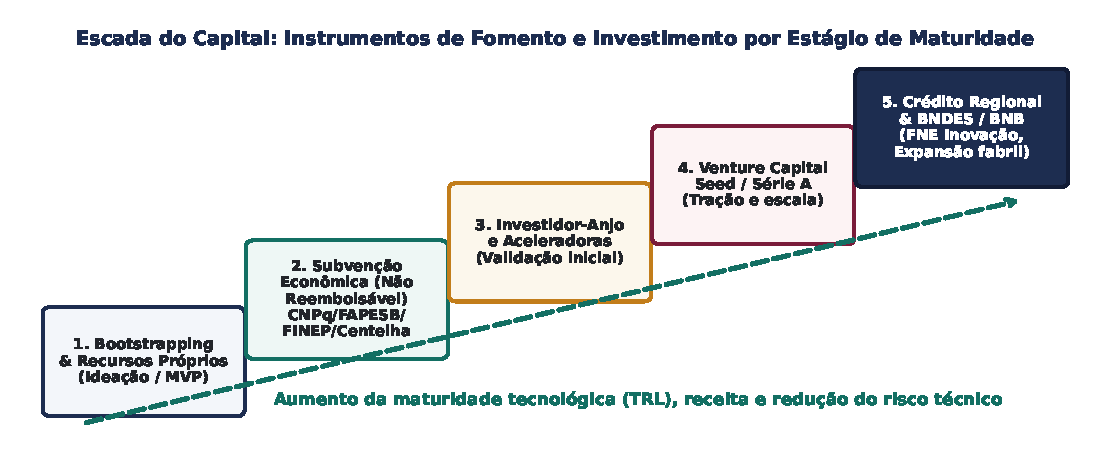
\includegraphics[width=0.94\textwidth]{figures/fig10_escada_capital.pdf}
  \caption{Escada do Capital para Empreendimentos de Base Tecnológica: alinhamento entre estágio TRL, instrumentos de fomento regional e diluição societária.}
  \label{fig:10_escada_capital}
\end{figure}

\section{Indicadores de Tração: MRR, \textit{Burn Rate} e \textit{Runway}}

Ao captar recursos na Escada do Capital, a gestão do tempo até a exaustão do caixa torna-se crítica. Três métricas operacionais governam a sobrevivência financeira de uma EBT em estágio inicial:

\begin{boxFormula}[Modelagem de Tração e Fôlego Financeiro: MRR, \textit{Burn Rate} e \textit{Runway}]
  \textbf{1. Receita Recorrente Mensal (MRR):} soma das assinaturas ou contratos mensais recorrentes ativos:
  \[
    \text{MRR} = \sum_{i=1}^{N} P_i = N_{\text{clientes}} \times \text{ARPU}.
  \]

  \textbf{2. Taxa de Queima de Caixa (\textit{Burn Rate}):} distingue-se entre queima bruta (\textit{Gross Burn}) e queima líquida (\textit{Net Burn}):
  \[
    \text{Gross Burn} = \text{Despesas Operacionais Mensais Totais},
  \]
  \[
    \text{Net Burn} = \text{Gross Burn} - \text{MRR}.
  \]
  Quando $\text{Net Burn} > 0$, a empresa consome reservas de caixa a cada mês. Quando $\text{MRR} \ge \text{Gross Burn}$, atinge-se o **ponto de equilíbrio operacional (\textit{break-even})**.

  \textbf{3. Fôlego Financeiro (\textit{Runway}):} número de meses de operação garantidos pelo caixa atual $K_0$, mantendo-se constante o \textit{Net Burn}:
  \[
    \text{Runway (meses)} = \frac{K_0}{\text{Net Burn}}.
  \]

  \textbf{4. Meses até o \textit{Break-Even} sob Crescimento Linear de Clientes:} se a empresa adiciona $\Delta N$ novos clientes líquidos por mês ao ticket $\text{ARPU}$, o incremento mensal de receita é $\Delta \text{MRR} = \Delta N \times \text{ARPU}$. O número de meses $t_{\text{BE}}$ para zerar o \textit{Net Burn} atual é:
  \[
    t_{\text{BE}} = \frac{\text{Net Burn}_{\text{atual}}}{\Delta \text{MRR}}.
  \]
\end{boxFormula}

\etapa{4}{Estudos de Caso e Exemplos Resolvidos em 7 Passos}

\begin{boxExemplo}{10.1}{Cálculo de MRR, \textit{Burn Rate}, \textit{Runway} e Tempo até \textit{Break-Even}}
  \passoEnunciado{Uma startup de automação hídrica sediada em Vitória da Conquista encerrou uma rodada combinada de subvenção estadual (FAPESB/Centelha) e aporte-anjo, dispondo de caixa imediato para escalar sua operação.}
  \passoDados{Caixa disponível atual ($K_0$): R\$\,360.000,00. Despesas operacionais mensais totais (folha técnica, insumos, nuvem e comercial): R\$\,48.000,00. Base ativa atual: 40 clientes pagantes com ticket médio ($\text{ARPU}$) de R\$\,450,00/mês. Ritmo líquido de aquisição projetado: 8 novos clientes pagantes por mês.}
  \passoPedido{Calcular o MRR atual, o \textit{Gross Burn}, o \textit{Net Burn}, o \textit{Runway} estático em meses e o tempo necessário para atingir o \textit{break-even} operacional.}
  \passoMetodo{Aplicação sequencial das equações de MRR, \textit{Burn Rate}, \textit{Runway} e crescimento linear de receita.}
  \passoContas{
    Primeiro, calcula-se o MRR atual e o \textit{Gross Burn}:
    \[
      \text{MRR} = 40 \times 450,00 = \text{R\$\,18.000,00/mês}, \qquad
      \text{Gross Burn} = \text{R\$\,48.000,00/mês}.
    \]
    Em seguida, calcula-se o \textit{Net Burn}:
    \[
      \text{Net Burn} = 48.000,00 - 18.000,00 = \text{R\$\,30.000,00/mês}.
    \]
    Com caixa de R\$\,360.000,00, o \textit{Runway} estático (caso a receita não cresça) é:
    \[
      \text{Runway} = \frac{360.000,00}{30.000,00} = 12{,}0\text{ meses}.
    \]
    Considerando a adição de 8 clientes líquidos/mês a R\$\,450,00, o ganho mensal de MRR é $\Delta \text{MRR} = 8 \times 450,00 = \text{R\$\,3.600,00/mês}$. O tempo até igualar as despesas de R\$\,48.000,00 (faltando R\$\,30.000,00 de MRR) é:
    \[
      t_{\text{BE}} = \frac{30.000,00}{3.600,00} \approx 8{,}33\text{ meses (no 9º mês)}.
    \]
  }
  \passoResposta{$\text{MRR} = \text{R\$\,18.000,00}$; $\text{Net Burn} = \text{R\$\,30.000,00/mês}$; $\text{Runway} = 12\text{ meses}$; \textit{break-even} atingido em 8{,}33 meses.}
  \passoVerificacao{Como $t_{\text{BE}} = 8{,}33 < 12{,}0$ meses de \textit{Runway} estático (e o consumo de caixa reduz a cada mês com o aumento do MRR), o caixa disponível é suficiente para levar a empresa ao equilíbrio operacional sem nova rodada emergencial.}
\end{boxExemplo}

\begin{boxExemplo}{10.2}{Subvenção Não Dilutiva vs. Capital Anjo na Escada do Capital}
  \passoEnunciado{Uma EBT em estágio TRL 5 precisa de R\$\,500.000,00 para concluir testes de campo e certificação de um biofertilizante. Ela compara duas rotas: (A) Subvenção Econômica (FINEP/FAPESB) com contrapartida financeira de 10\% dos sócios; ou (B) Captação integral de R\$\,500.000,00 com investidor-anjo em troca de 15\% de participação societária.}
  \passoDados{Valor total requerido: R\$\,500.000,00. Rota A: 90\% subvenção não reembolsável + 10\% contrapartida própria, 0\% de diluição. Rota B: 100\% capital anjo, 15\% de diluição societária.}
  \passoPedido{Calcular o valor da contrapartida própria na Rota A, o \textit{valuation post-money} implícito na Rota B e o custo societário evitado caso a empresa venha a valer R\$\,10.000.000,00 em 5 anos.}
  \passoMetodo{Análise comparativa de diluição societária e \textit{valuation} implícito na Escada do Capital.}
  \passoContas{
    Na Rota A, a subvenção aporta $500.000 \times 0{,}90 = \text{R\$\,450.000,00}$ e os sócios aportam $500.000 \times 0{,}10 = \text{R\$\,50.000,00}$ de contrapartida, mantendo 100\% das quotas.
    Na Rota B, se R\$\,500.000,00 compram 15\% ($0{,}15$) da empresa, o valor total pós-aporte (\textit{post-money}) é:
    \[
      V_{\text{post-money}} = \frac{500.000,00}{0{,}15} = \text{R\$\,3.333.333,33}.
    \]
    Se a empresa alcançar \textit{valuation} de R\$\,10.000.000,00 no Ano 5, os 15\% cedidos na Rota B equivalerão a $10.000.000 \times 0{,}15 = \text{R\$\,1.500.000,00}$ transferidos ao investidor em troca dos R\$\,500.000,00 iniciais.
  }
  \passoResposta{A Rota A exige R\$\,50.000,00 de contrapartida e preserva 100\% do controle; a Rota B implica \textit{valuation post-money} de R\$\,3,33 milhões e cede 15\% (equivalente a R\$\,1,5 milhão em um cenário futuro de R\$\,10 milhões).}
  \passoVerificacao{O cálculo demonstra por que instrumentos não dilutivos (FAPESB, FINEP, Centelha) devem ser priorizados nos estágios TRL 3–6 antes da abertura de capital societário.}
\end{boxExemplo}

\begin{boxExemplo}{10.3}{Crédito Regional BNB / FNE Inovação para Implantação Produtiva}
  \passoEnunciado{Uma agroindústria tecnológica no Semiárido baiano atingiu TRL 8 e precisa de R\$\,400.000,00 para instalar uma linha de beneficiamento de frutas nativas.}
  \passoDados{Financiamento via FNE Inovação (Banco do Nordeste): R\$\,400.000,00, taxa efetiva de 8{,}5\% ao ano, carência de 24 meses (pagando apenas juros sem amortização do principal durante a carência) e amortização nos 60 meses seguintes.}
  \passoPedido{Calcular o encargo anual de juros durante o período de carência e compará-lo com uma linha comercial de mercado a 20\% ao ano.}
  \passoMetodo{Cálculo de juros anuais sobre saldo devedor integral durante a carência e diferencial de custo financeiro.}
  \passoContas{
    No FNE Inovação (8{,}5\% a.a.):
    \[
      J_{\text{FNE/ano}} = 400.000,00 \times 0{,}085 = \text{R\$\,34.000,00/ano} \quad (\text{R\$\,68.000,00 nos 2 anos de carência}).
    \]
    Na linha comercial (20\% a.a.):
    \[
      J_{\text{comercial/ano}} = 400.000,00 \times 0{,}20 = \text{R\$\,80.000,00/ano} \quad (\text{R\$\,160.000,00 nos 2 anos de carência}).
    \]
    Economia financeira gerada apenas durante os 24 meses de carência:
    \[
      \text{Economia} = 160.000,00 - 68.000,00 = \text{R\$\,92.000,00}.
    \]
  }
  \passoResposta{O crédito FNE Inovação gera encargo de R\$\,34.000,00/ano na carência, economizando R\$\,92.000,00 em juros nos dois primeiros anos frente ao crédito comercial.}
  \passoVerificacao{A carência de 24 meses protege o fluxo de caixa durante a montagem da planta industrial, desde que o projeto já possua demanda contratada para iniciar a amortização no Ano 3.}
\end{boxExemplo}

\begin{boxExemplo}{10.4}{Escolha do Formato de Planejamento Conforme o Interlocutor}
  \passoEnunciado{Os fundadores de uma startup de monitoramento ambiental foram convidados na mesma semana para: (1) uma rodada rápida de 5 minutos com investidores-anjo; (2) submissão preliminar ao Programa Centelha; e (3) análise de crédito de implantação no BNDES/BNB.}
  \passoDados{Tempo e exigências de cada interlocutor: apresentação oral de 5 minutos; formulário de triagem de até 3 páginas; e dossiê de engenharia econômico-financeira com garantias e cronograma.}
  \passoPedido{Associar cada demanda ao formato adequado (Plano Completo, Sumário Executivo ou \textit{Pitch Deck}) e indicar o foco central de cada documento.}
  \passoMetodo{Alinhamento entre instrumento de comunicação estratégica e critério de decisão do financiador.}
  \passoContas{
    (1) Rodada de 5 minutos $\to$ \textbf{\textit{Pitch Deck}} (10–12 slides visuais focados em dor, tração, TAM/SAM/SOM e equipe); (2) Triagem no Programa Centelha $\to$ \textbf{Sumário Executivo} (2–4 páginas com mérito inovador, grau de novidade/PI e orçamento enxuto); (3) Crédito no BNDES/BNB $\to$ \textbf{Plano de Negócio Completo} (projeção de fluxo de caixa, capacidade de pagamento, garantias e impacto regional).
  }
  \passoResposta{(1) \textit{Pitch Deck}; (2) Sumário Executivo; (3) Plano de Negócio Completo.}
  \passoVerificacao{Enviar um plano de 80 páginas para um investidor-anjo na primeira abordagem ou tentar aprovar crédito bancário apenas com slides de \textit{pitch} resulta em rejeição imediata.}
\end{boxExemplo}

\begin{boxExemplo}{10.5}{Timing da Captação e Preservação de Controle Acionário}
  \passoEnunciado{Uma EBT precisa captar R\$\,600.000,00. Se captar hoje com MRR = R\$\,0 (pré-validação), o fundo avalia a empresa em R\$\,1.200.000,00 (\textit{pre-money}). Se usar R\$\,120.000,00 de subvenção estadual primeiro para atingir MRR = R\$\,25.000,00/mês, o fundo passará a avaliá-la em R\$\,3.400.000,00 (\textit{pre-money}).}
  \passoDados{Captação alvo: R\$\,600.000,00. Cenário 1 (\textit{pre-money} = R\$\,1,2M). Cenário 2 (\textit{pre-money} = R\$\,3,4M).}
  \passoPedido{Calcular a diluição societária em cada cenário ($\% \text{ cedido} = \frac{\text{Aporte}}{\text{Pre-money} + \text{Aporte}}$).}
  \passoMetodo{Cálculo de participação acionária pós-aporte (\textit{post-money}).}
  \passoContas{
    Cenário 1 (antes da tração):
    \[
      \text{Diluição}_1 = \frac{600.000}{1.200.000 + 600.000} = \frac{600.000}{1.800.000} = 33{,}33\%.
    \]
    Cenário 2 (após validação com subvenção):
    \[
      \text{Diluição}_2 = \frac{600.000}{3.400.000 + 600.000} = \frac{600.000}{4.000.000} = 15{,}00\%.
    \]
    A validação prévia com recurso não dilutivo economizou $33{,}33\% - 15{,}00\% = 18{,}33$ pontos percentuais de participação dos fundadores.
  }
  \passoResposta{A diluição cai de 33{,}33\% para 15{,}00\%, preservando 18{,}33\% adicionais da empresa para os empreendedores.}
  \passoVerificacao{Subir um degrau na Escada do Capital usando fomento público antes de buscar \textit{equity} multiplica o poder de barganha dos fundadores.}
\end{boxExemplo}

\etapa{5}{Armadilhas Conceituais e Erros Mais Comuns}

\begin{boxErro}[Erro 1 — Confundir \textit{Gross Burn} com \textit{Net Burn} ao Calcular o \textit{Runway}]
  Dividir o caixa disponível apenas pelas despesas totais (\textit{Gross Burn}) ignora as entradas de receita mensal (MRR), subestimando o fôlego real; inversamente, esquecer despesas não mensais (13º salário, impostos trimestrais ou manutenção anual) superestima o \textit{Runway}.
\end{boxErro}

\begin{boxErro}[Erro 2 — Captar Crédito Bancário Reembolsável em TRL 3 ou 4]
  Assumir dívida com juros e prazo fixo antes de ter receita previsível transfere o risco tecnológico integralmente para o patrimônio pessoal dos sócios. Em TRL 3–5, o instrumento adequado é subvenção não reembolsável ou capital paciente, nunca dívida comercial.
\end{boxErro}

\begin{boxErro}[Erro 3 — Tratar Subvenção Econômica como Dinheiro Livre de Prestação de Contas]
  Embora a subvenção (CNPq, FAPESB, FINEP) não exija devolução do principal nem participação societária, ela impõe execução estrita ao plano de trabalho aprovado, rubricas específicas, contrapartidas e prestação de contas físico-financeira rigorosa.
\end{boxErro}

\begin{boxErro}[Erro 4 — Esperar o Caixa Chegar a 2 Meses de \textit{Runway} para Iniciar Captação]
  Processos de aprovação em editais públicos, bancos regionais (BNB/BNDES) ou fundos de \textit{Venture Capital} levam tipicamente de 6 a 12 meses. Iniciar a busca por recursos apenas quando o \textit{Runway} é inferior a 6 meses coloca a empresa em posição de insolvência ou negociação desfavorável.
\end{boxErro}

\etapa{6}{Lista de Exercícios (15 Questões em 3 Níveis)}

\textbf{Nível 1 — Fundamentos Conceituais (Questões 1 a 5)}

\begin{enumerate}[leftmargin=1.5em, itemsep=6pt]
  \item Diferencie o objetivo, a extensão e o público-alvo do \textit{Pitch Deck}, do Sumário Executivo e do Plano de Negócio Completo.
  \espacoResolucao[1.8cm]

  \item Explique a diferença entre capital não dilutivo e capital dilutivo (\textit{equity}) na Escada do Capital para EBTs.
  \espacoResolucao[1.8cm]

  \item Indique a vocação principal de cada instrumento no ecossistema brasileiro e baiano: Programa Centelha, FAPESB, FINEP, BNB/FNE Inovação e BNDES.
  \espacoResolucao[1.8cm]

  \item Defina MRR, \textit{Gross Burn Rate}, \textit{Net Burn Rate} e \textit{Runway}, explicando em que condição o \textit{Net Burn} torna-se zero ou negativo.
  \espacoResolucao[1.8cm]

  \item Por que um investidor-anjo costuma ser classificado como \textit{smart money} e em que estágio TRL sua entrada faz mais sentido?
  \espacoResolucao[1.8cm]

  \item \textbf{(Nível 2 — Aplicações Numéricas)} Uma startup possui 60 clientes pagando assinatura mensal de R\$\,350,00 e despesas operacionais mensais totais de R\$\,39.000,00. Seu caixa atual é de R\$\,216.000,00. Calcule o MRR, o \textit{Net Burn} e o \textit{Runway} estático em meses.
  \espacoResolucao[2.2cm]

  \item No exercício anterior, se a startup conquistar 6 novos clientes líquidos por mês ao mesmo ticket de R\$\,350,00, em quantos meses atingirá o \textit{break-even} operacional?
  \espacoResolucao[2.2cm]

  \item Uma EBT aprovou projeto de R\$\,300.000,00 em edital de subvenção econômica que exige 20\% de contrapartida econômica ou financeira da empresa. Qual o valor repassado pela agência de fomento e qual o valor da contrapartida?
  \espacoResolucao[2.1cm]

  \item Um investidor-anjo aporta R\$\,250.000,00 por 12{,}5\% de participação societária em uma startup tecnológica. Qual o \textit{valuation post-money} e o \textit{valuation pre-money} da operação?
  \espacoResolucao[2.2cm]

  \item Uma empresa tem despesas operacionais de R\$\,55.000,00/mês, MRR de R\$\,25.000,00/mês e caixa de R\$\,180.000,00. Caso reduza suas despesas em R\$\,10.000,00/mês mantendo o MRR constante, em quantos meses aumentará seu \textit{Runway}?
  \espacoResolucao[2.2cm]

  \item \textbf{(Nível 3 — Análise Territorial e Estratégica)} Descreva uma sequência ótima na Escada do Capital para levar uma tecnologia agroindustrial desenvolvida na UEFS do nível TRL 3 até a escala industrial (TRL 9) no interior da Bahia, articulando ao menos três fontes distintas de recursos.
  \espacoResolucao[2.3cm]

  \item Uma empresa pode captar R\$\,400.000,00 via \textit{Venture Capital} cedendo 20\% do capital ou combinar R\$\,250.000,00 de subvenção (0\% diluição) com R\$\,150.000,00 de empréstimo FNE Inovação. Analise os riscos e benefícios de cada alternativa sob a ótica da diluição e da pressão sobre o fluxo de caixa.
  \espacoResolucao[2.3cm]

  \item Explique por que o \textit{Runway} mínimo recomendado para iniciar uma nova rodada de captação ou submissão a crédito estruturado é de 9 a 12 meses.
  \espacoResolucao[2.1cm]

  \item Uma startup tem caixa de R\$\,240.000,00, \textit{Gross Burn} de R\$\,50.000,00/mês e MRR de R\$\,20.000,00/mês. Ao longo dos próximos 3 meses, o MRR cresce R\$\,5.000,00 por mês (Mês 1 = 25.000; Mês 2 = 30.000; Mês 3 = 35.000). Calcule o saldo exato de caixa ao final do Mês 3.
  \espacoResolucao[2.4cm]

  \item Estruture o roteiro de um \textit{Pitch Deck} de 10 slides para submissão de um projeto territorial de bioeconomia a um comitê regional de fomento.
  \espacoResolucao[2.3cm]
\end{enumerate}

\etapa{7}{Questões Autorais Estilo Pós-Graduação / Concursos de CT\&I}

\begin{enumerate}[leftmargin=1.5em, itemsep=6pt]
  \item \textbf{(Estilo ANPAD / Finanças Empreendedoras)} Uma empresa de base tecnológica apresenta caixa disponível de R\$\,420.000,00, despesas operacionais mensais de R\$\,65.000,00 e receita recorrente mensal (MRR) de R\$\,30.000,00. Considerando essas variáveis constantes, o \textit{Net Burn Rate} e o \textit{Runway} da empresa são, respectivamente:
  \begin{alternativas}
    \item R\$\,65.000,00/mês e 6{,}46 meses.
    \item R\$\,35.000,00/mês e 12{,}0 meses.
    \item R\$\,30.000,00/mês e 14{,}0 meses.
    \item R\$\,35.000,00/mês e 6{,}46 meses.
    \item R\$\,95.000,00/mês e 4{,}42 meses.
  \end{alternativas}
  \espacoResolucao[1.5cm]

  \item \textbf{(Estilo Concurso Analista de Fomento — FINEP/BNDES)} Relacione os instrumentos financeiros às suas características na Escada do Capital:
  I. Subvenção econômica (FINEP/FAPESB/Centelha) atua no compartilhamento de risco tecnológico pré-comercial sem diluição societária nem devolução financeira do principal.
  II. O crédito regional (como o FNE Inovação do BNB) dispensa capacidade de pagamento porque atua na mesma lógica de fundo perdido da subvenção.
  III. O \textit{Venture Capital} busca empresas com modelo validado e alto potencial de escala, aceitando risco de negócio em troca de participação societária.
  Assinale a alternativa correta:
  \begin{alternativas}
    \item Apenas I está correta.
    \item Apenas II está correta.
    \item Apenas I e III estão corretas.
    \item Apenas II e III estão corretas.
    \item I, II e III estão corretas.
  \end{alternativas}
  \espacoResolucao[1.5cm]

  \item \textbf{(Estilo Discursiva — PPGPT)} Explique por que a ausência de coordenação entre instrumentos não reembolsáveis (CNPq/FAPESB/FINEP) e instrumentos de crédito regional (BNB/BNDES) pode perpetuar o Vale da Morte Tecnológico em regiões periféricas.
  \espacoResolucao[2.3cm]
\end{enumerate}

\begin{boxDica}[Contraponto Crítico e Prática Territorial (AV3)]
  No Projeto Final (AV3), evite indicar genericamente ``buscar financiamento''. Especifique exatamente qual degrau da Escada do Capital corresponde ao estágio TRL atual do seu projeto (por exemplo, Centelha/FAPESB para prototipagem TRL 4–5 ou FNE Inovação para planta TRL 8), apresente o \textit{Net Burn} mensal estimado e o \textit{Runway} necessário para atingir o ponto de equilíbrio.
\end{boxDica}

\clearpage
\etapa{8}{Gabarito Integralmente Comentado (Exercícios 1 a 18)}

\begin{boxGabarito}[Resolução Completa dos Exercícios da Etapa 6 (1 a 15) e Etapa 7 (16 a 18)]
  \begin{enumerate}[leftmargin=1.5em, itemsep=4pt]
    \item \textbf{Resposta:} \textit{Pitch Deck} (10–15 slides) visa atrair interesse inicial de investidores/bancas; Sumário Executivo (2–4 páginas) sintetiza mérito e orçamento para triagem de editais; Plano Completo detalha engenharia, mercado, localização e projeções financeiras para crédito e governança.
    \item \textbf{Resposta:} Não dilutivo aporta recursos sem ceder quotas da empresa (subvenção, prêmios); dilutivo (\textit{equity}) troca capital por participação societária (anjo, VC).
    \item \textbf{Resposta:} Centelha: ideação e validação inicial; FAPESB: fomento científico e inovação estadual na Bahia; FINEP: subvenção e financiamento à inovação tecnológica nacional; BNB/FNE Inovação: crédito regional subsidiado para o Nordeste; BNDES: crédito de longo prazo e infraestrutura produtiva.
    \item \textbf{Resposta:} MRR é a receita recorrente mensal; \textit{Gross Burn} são as despesas operacionais totais; \textit{Net Burn} é $\text{Despesas} - \text{MRR}$; \textit{Runway} é $\text{Caixa} / \text{Net Burn}$. Quando $\text{MRR} \ge \text{Gross Burn}$, o \textit{Net Burn} zera ou torna-se negativo (geração líquida de caixa).
    \item \textbf{Resposta:} Porque além de dinheiro, o anjo aporta mentoria, governança e rede de clientes; sua entrada é mais adequada entre TRL 5 e 7, após prova de conceito inicial.
    \item \textbf{Resposta:} $\text{MRR} = 60 \times 350 = \text{R\$\,21.000,00}$. $\text{Net Burn} = 39.000 - 21.000 = \text{R\$\,18.000,00/mês}$. $\text{Runway} = 216.000 / 18.000 = 12{,}0\text{ meses}$.
    \item \textbf{Resposta:} Incremento mensal de MRR $= 6 \times 350 = \text{R\$\,2.100,00/mês}$. Faltam R\$\,18.000,00 de MRR para igualar R\$\,39.000,00. Logo, $t_{\text{BE}} = 18.000 / 2.100 \approx 8{,}57\text{ meses}$ (no 9º mês).
    \item \textbf{Resposta:} Se o projeto total é R\$\,300.000,00 e a contrapartida é 20\% sobre esse valor, a contrapartida é R\$\,60.000,00 e o repasse da agência é R\$\,240.000,00 (caso os 20\% sejam calculados adicionalmente sobre o repasse de R\$\,300.000,00, a contrapartida será de R\$\,60.000,00 totalizando R\$\,360.000,00; convém sempre verificar a regra do edital).
    \item \textbf{Resposta:} $V_{\text{post-money}} = 250.000 / 0{,}125 = \text{R\$\,2.000.000,00}$. $V_{\text{pre-money}} = 2.000.000 - 250.000 = \text{R\$\,1.750.000,00}$.
    \item \textbf{Resposta:} Antes: $\text{Net Burn} = 55.000 - 25.000 = \text{R\$\,30.000,00}$; $\text{Runway} = 180.000 / 30.000 = 6{,}0\text{ meses}$. Depois: $\text{Net Burn} = 45.000 - 25.000 = \text{R\$\,20.000,00}$; $\text{Runway} = 180.000 / 20.000 = 9{,}0\text{ meses}$. Aumento de $3{,}0\text{ meses}$ ($+50\%$).
    \item \textbf{Resposta:} TRL 3–4: bolsa/edital CNPq ou FAPESB e Programa Centelha; TRL 5–7: subvenção FINEP Tecnova + investidor-anjo para validação comercial; TRL 8–9: crédito FNE Inovação (BNB) para montagem da planta agroindustrial.
    \item \textbf{Resposta:} VC (20\%): sem dívida fixa, mas alta diluição permanente. Subvenção + FNE: preserva 100\% do controle societário, porém exige contrapartida/prestação de contas na subvenção e capacidade de pagamento de juros/principal no crédito FNE.
    \item \textbf{Resposta:} Porque editais, análises de crédito e rodadas de investimento duram tipicamente de 6 a 12 meses entre submissão, diligência e desembolso; negociar com menos de 6 meses reduz o poder de barganha e gera risco de quebra.
    \item \textbf{Resposta:} Mês 1: $\text{Net Burn}_1 = 50.000 - 25.000 = 25.000 \implies \text{Caixa}_1 = 240.000 - 25.000 = 215.000$. Mês 2: $\text{Net Burn}_2 = 50.000 - 30.000 = 20.000 \implies \text{Caixa}_2 = 215.000 - 20.000 = 195.000$. Mês 3: $\text{Net Burn}_3 = 50.000 - 35.000 = 15.000 \implies \text{Caixa}_3 = \text{R\$\,180.000,00}$.
    \item \textbf{Resposta:} 1. Capa/Propósito; 2. Dor territorial; 3. Solução tecnológica; 4. Mercado (TAM/SAM/SOM); 5. Modelo de Negócio (BMC); 6. Tração/MVP; 7. Diferencial/PI; 8. Impacto Territorial; 9. Equipe; 10. Necessidade de Capital e Uso dos Recursos.
    \item \textbf{Questão 16 (Etapa 7) — Gabarito: (B).} $\text{Net Burn} = 65.000 - 30.000 = \text{R\$\,35.000,00/mês}$; $\text{Runway} = 420.000 / 35.000 = 12{,}0\text{ meses}$.
    \item \textbf{Questão 17 (Etapa 7) — Gabarito: (C).} II é falsa porque crédito regional (FNE Inovação) é reembolsável e exige análise de capacidade de pagamento e garantias.
    \item \textbf{Questão 18 (Etapa 7) — Espelho Discursivo:} Deve explicar que, se o fomento não reembolsável financia apenas a pesquisa (TRL 1–3) e o crédito regional exige histórico de faturamento e garantias reais (TRL 8–9), cria-se um hiato de financiamento entre TRL 4 e 7 que bloqueia a transição de tecnologias locais para a escala produtiva.
  \end{enumerate}
\end{boxGabarito}

\begin{boxResumo}
  \begin{itemize}[leftmargin=1.4em, itemsep=2pt]
    \item O formato do planejamento deve adequar-se ao interlocutor (\textit{Pitch Deck}, Sumário Executivo ou Plano Completo).
    \item A Escada do Capital alinha risco tecnológico (TRL) e fonte de financiamento: \textit{bootstrapping} e subvenção nos estágios iniciais, capital de risco na validação/escala e crédito regional (BNB/BNDES) na implantação produtiva.
    \item O monitoramento contínuo de MRR, \textit{Net Burn} e \textit{Runway} assegura que a captação ocorra antes da zona crítica de caixa.
  \end{itemize}
\end{boxResumo}

\begin{boxTeste}
  \begin{enumerate}[leftmargin=1.5em, itemsep=4pt]
    \item (\V/\F) Um \textit{Pitch Deck} de 10 slides substitui integralmente o Plano de Negócio Completo na solicitação de crédito industrial junto ao BNB ou BNDES.
    \item (\V/\F) A subvenção econômica (CNPq/FAPESB/FINEP) é considerada capital não dilutivo porque não exige cessão de participação societária.
    \item (\V/\F) Se uma startup possui $\text{MRR} = \text{R\$\,20.000,00}$, despesas mensais de R\$\,50.000,00 e caixa de R\$\,150.000,00, seu \textit{Runway} estático é de 5 meses.
    \item (\V/\F) Captar \textit{Venture Capital} antes de validar o MVP e o modelo de negócio tende a provocar maior diluição societária dos fundadores.
  \end{enumerate}
  \begin{boxGabarito}[Respostas do Checkpoint — Capítulo 10]
    \textbf{1: \F} (Bancos de fomento exigem plano completo e análise de garantias). \quad \textbf{2: \V}. \quad \textbf{3: \V} ($\text{Net Burn} = 30.000$; $150.000 / 30.000 = 5\text{ meses}$). \quad \textbf{4: \V}.
  \end{boxGabarito}
\end{boxTeste}
